\section{Periodic Repetition}
\label{peridodic_section}
\subsection{Improvement Goals}
A description for periodic boundary conditions is given in \cref{pbc_explain} regarding how a small simulation box simulates a subset of an infinite lattice. It may be useful to visualise a larger subset of this infinite lattice by repeating the simulation box a number of times. Additionally, the capability of repeating a smaller system is useful for producing a realistic, much larger configuration for testing the performance of WebMGA with increased molecule counts due to the lack of availability of real test configurations of such sizes.

\subsection{WebMGA 3.0 Implementation}
A few modifications needed to be made to implement this feature.

First, the ``reference'' tab in the side menu was modified to include inputs for the repeat count in the `x' `y' and `z' directions. With a value of zero, there should be only a single instance of the configuration along the corresponding axis. Setting to one adds a repeat in the positive and negative direction along the axis, with bounding box faces touching (i.e. with a value of 0, there will be 1 instance of the configuration, with 1 there will be 3 instances, 2 there will be 5 instances etc.). When multiple directions have a value larger than 0, the configurations are repeated such that a single large box is produced (i.e. it is ensured there are no gaps, for example a configuration of $(1,1,1)$ will give a box of dimensions $3\times 3\times 3$ with $27$ total instances of the initial configuration).

Repetition of the configuration was implemented by changing the ``setState'' method. After building a configuration, the repeats parameters are read and each molecule is duplicated $x \times y \times z$ times according to the following pseudocode where `unitBoxSize' is a 3D vector defining half each dimension of the configuration's unit box,

\begin{lstlisting}
  FOR molecule of molecules
    FOR x=-X to X
      FOR y=-Y to Y
        FOR z=-Z to Z
          newMolecule = molecule.clone
          newMolecule.position += unitBoxSize * [x, y, z]
          scene.add(newMolecule)
        end FOR
      end FOR
    end FOR
  end FOR
\end{lstlisting}.

After implementing this feature, it was found that when changes were made to the configuration the duplicated molecules were not updated. This was fixed by modifying the molecule set generation function to remove and then reduplicate the extra molecules upon changes.

\begin{figure}
  \begin{center}
    \begin{subfigure}{0.3\textwidth}
      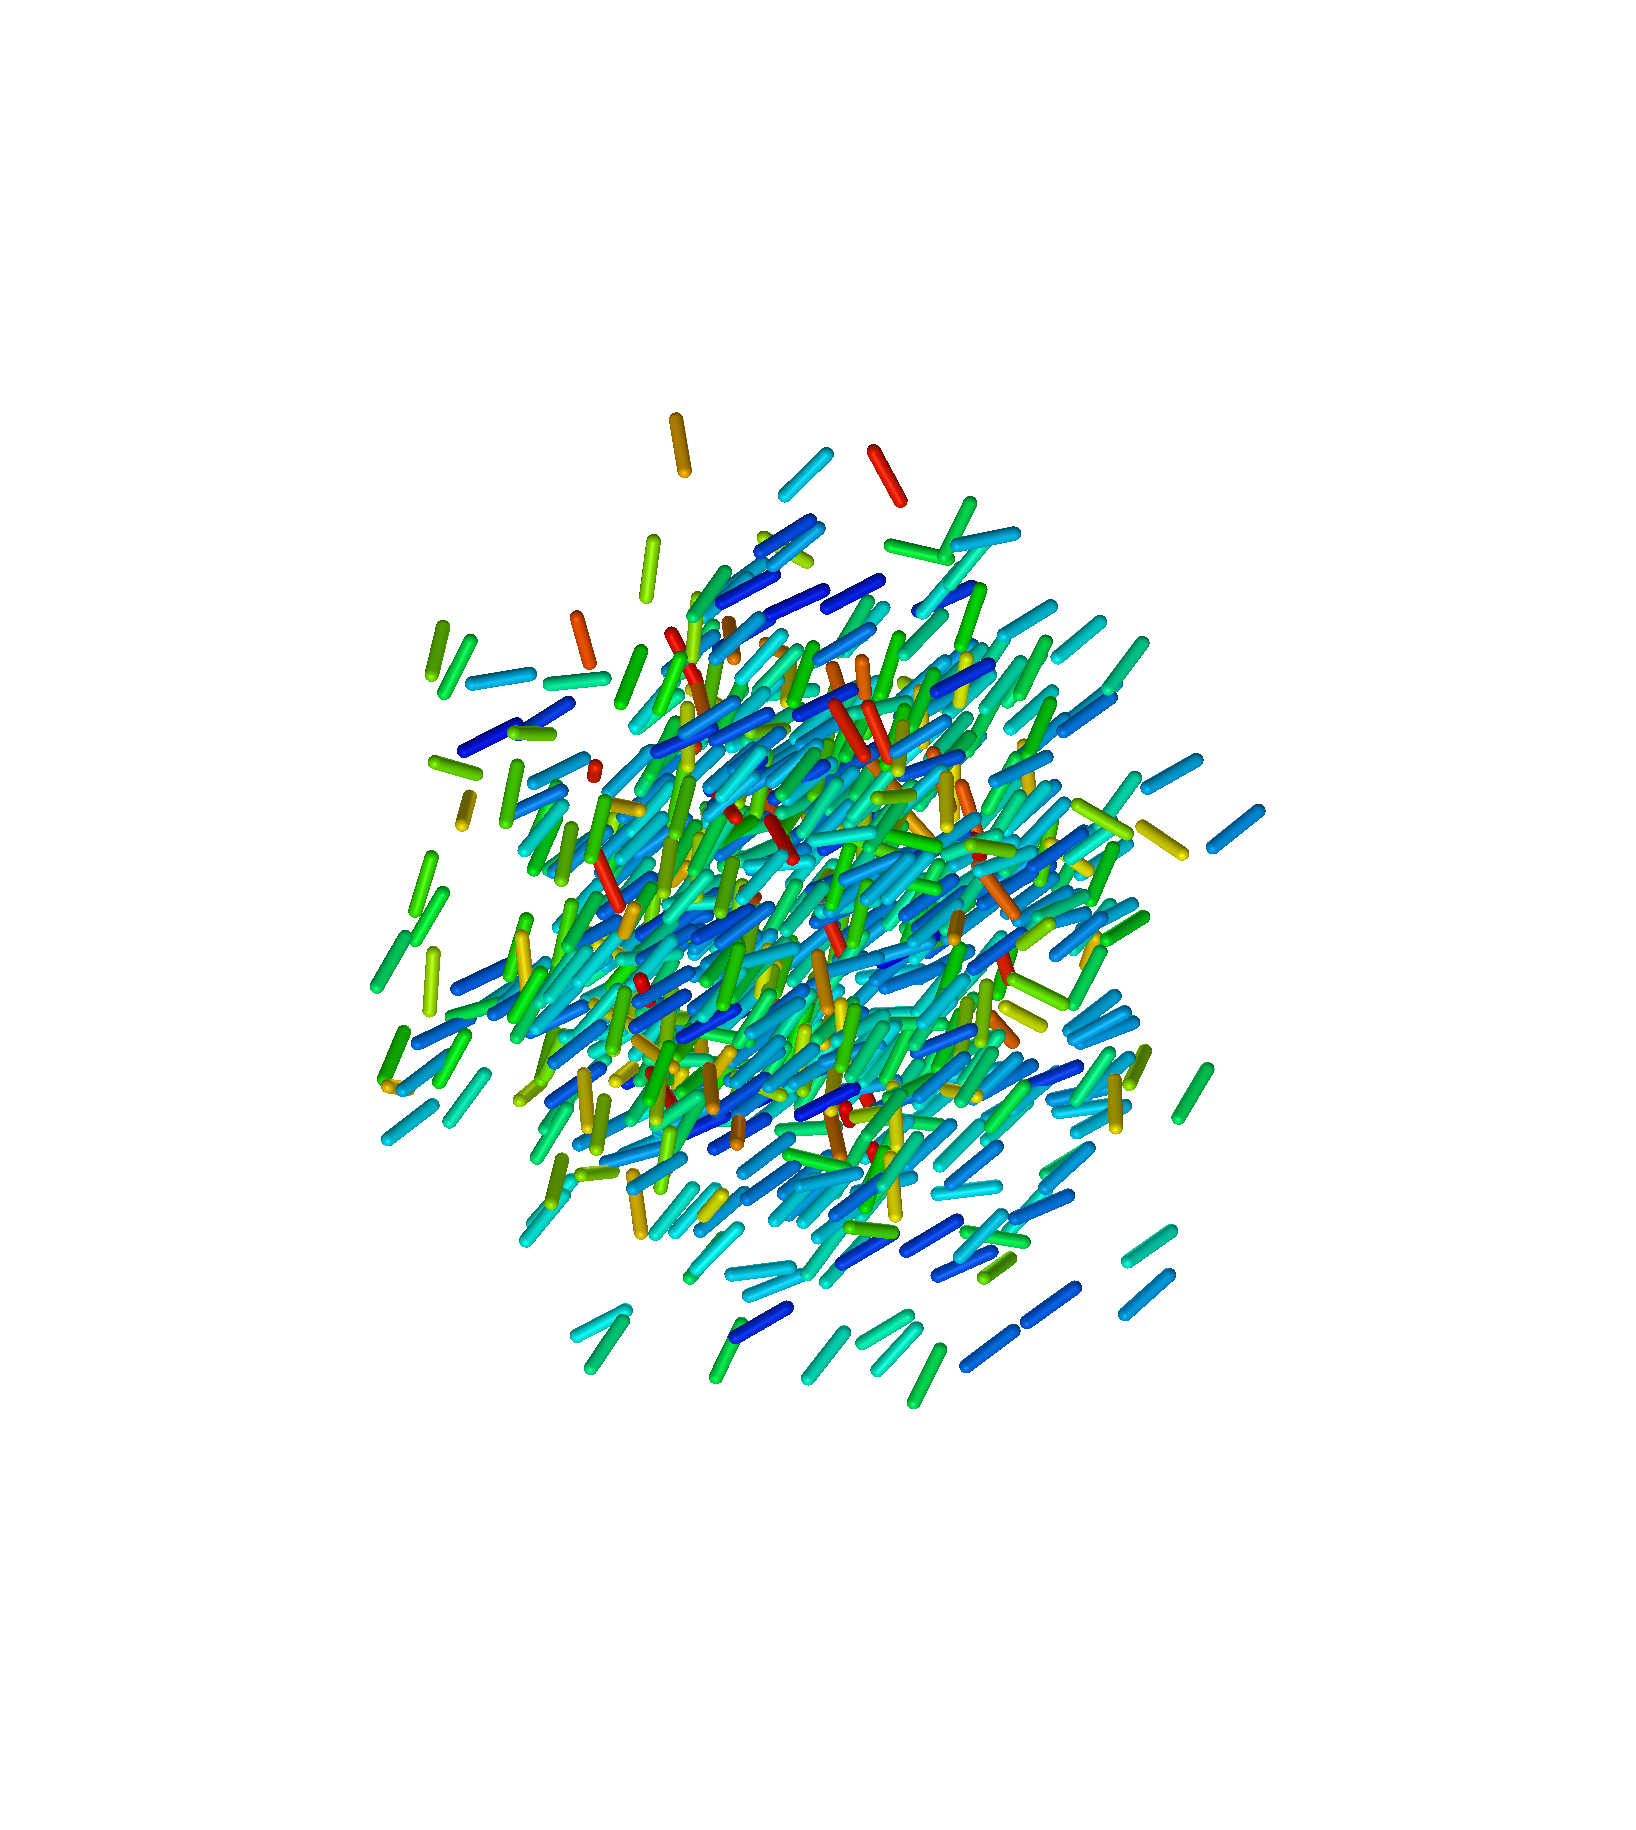
\includegraphics[width=\textwidth]{assets/images/periodic/1}
      \caption{$(0,0,0)$}
      \label{fig:periodic_1}
    \end{subfigure}
        \begin{subfigure}{0.3\textwidth}
      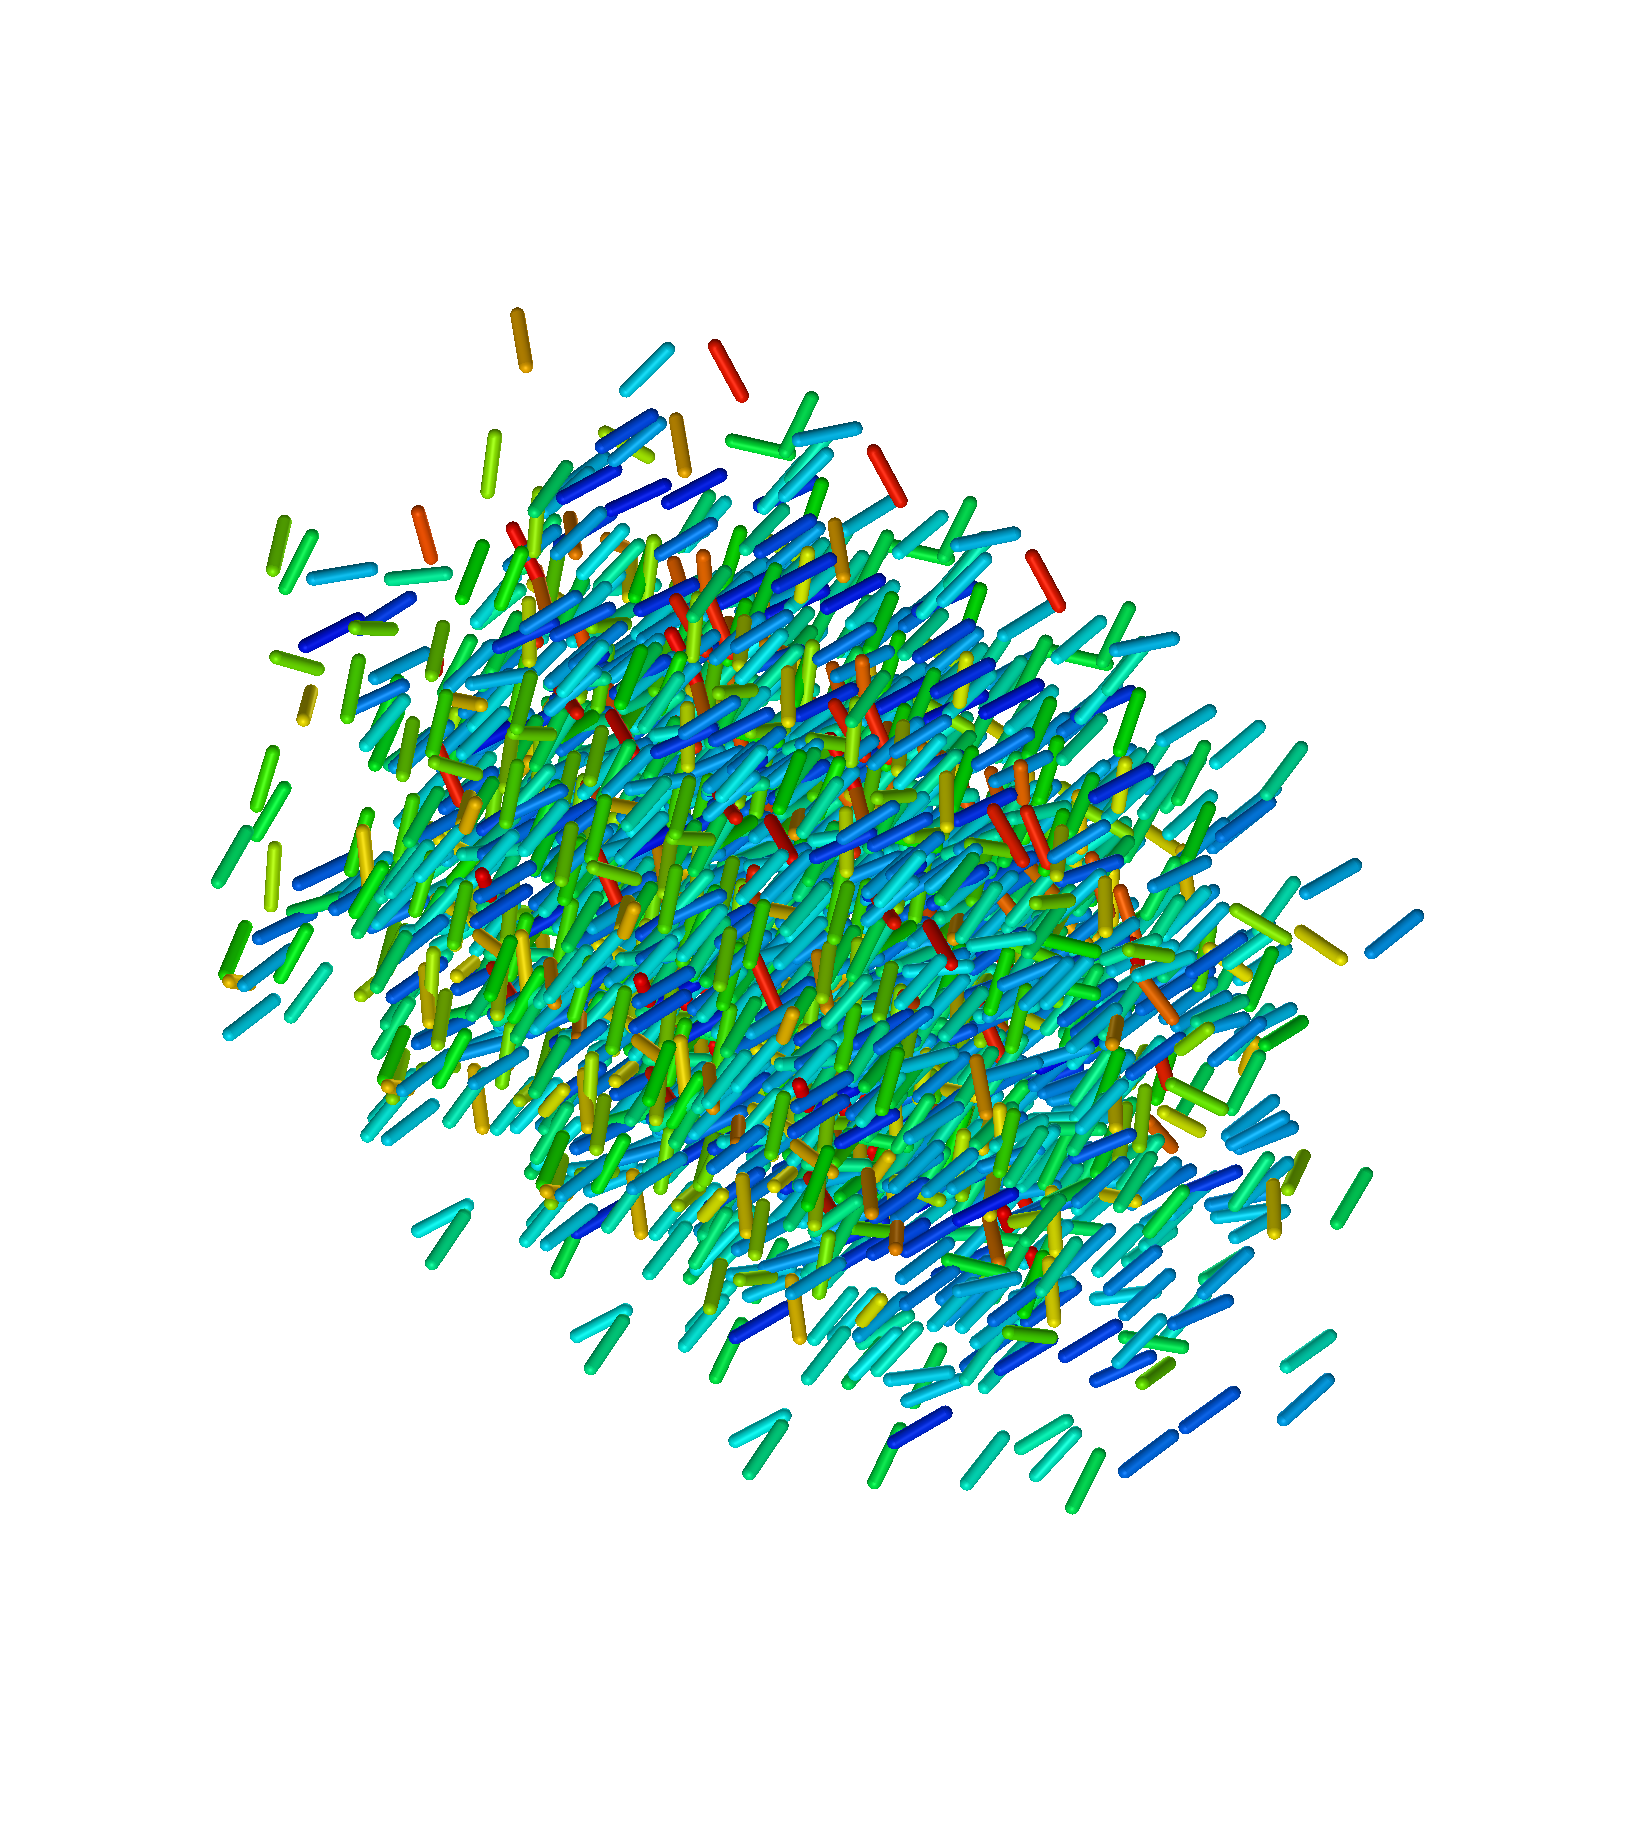
\includegraphics[width=\textwidth]{assets/images/periodic/2}
      \caption{$(1,0,0)$}
      \label{fig:periodic_2}
    \end{subfigure}
        \begin{subfigure}{0.3\textwidth}
      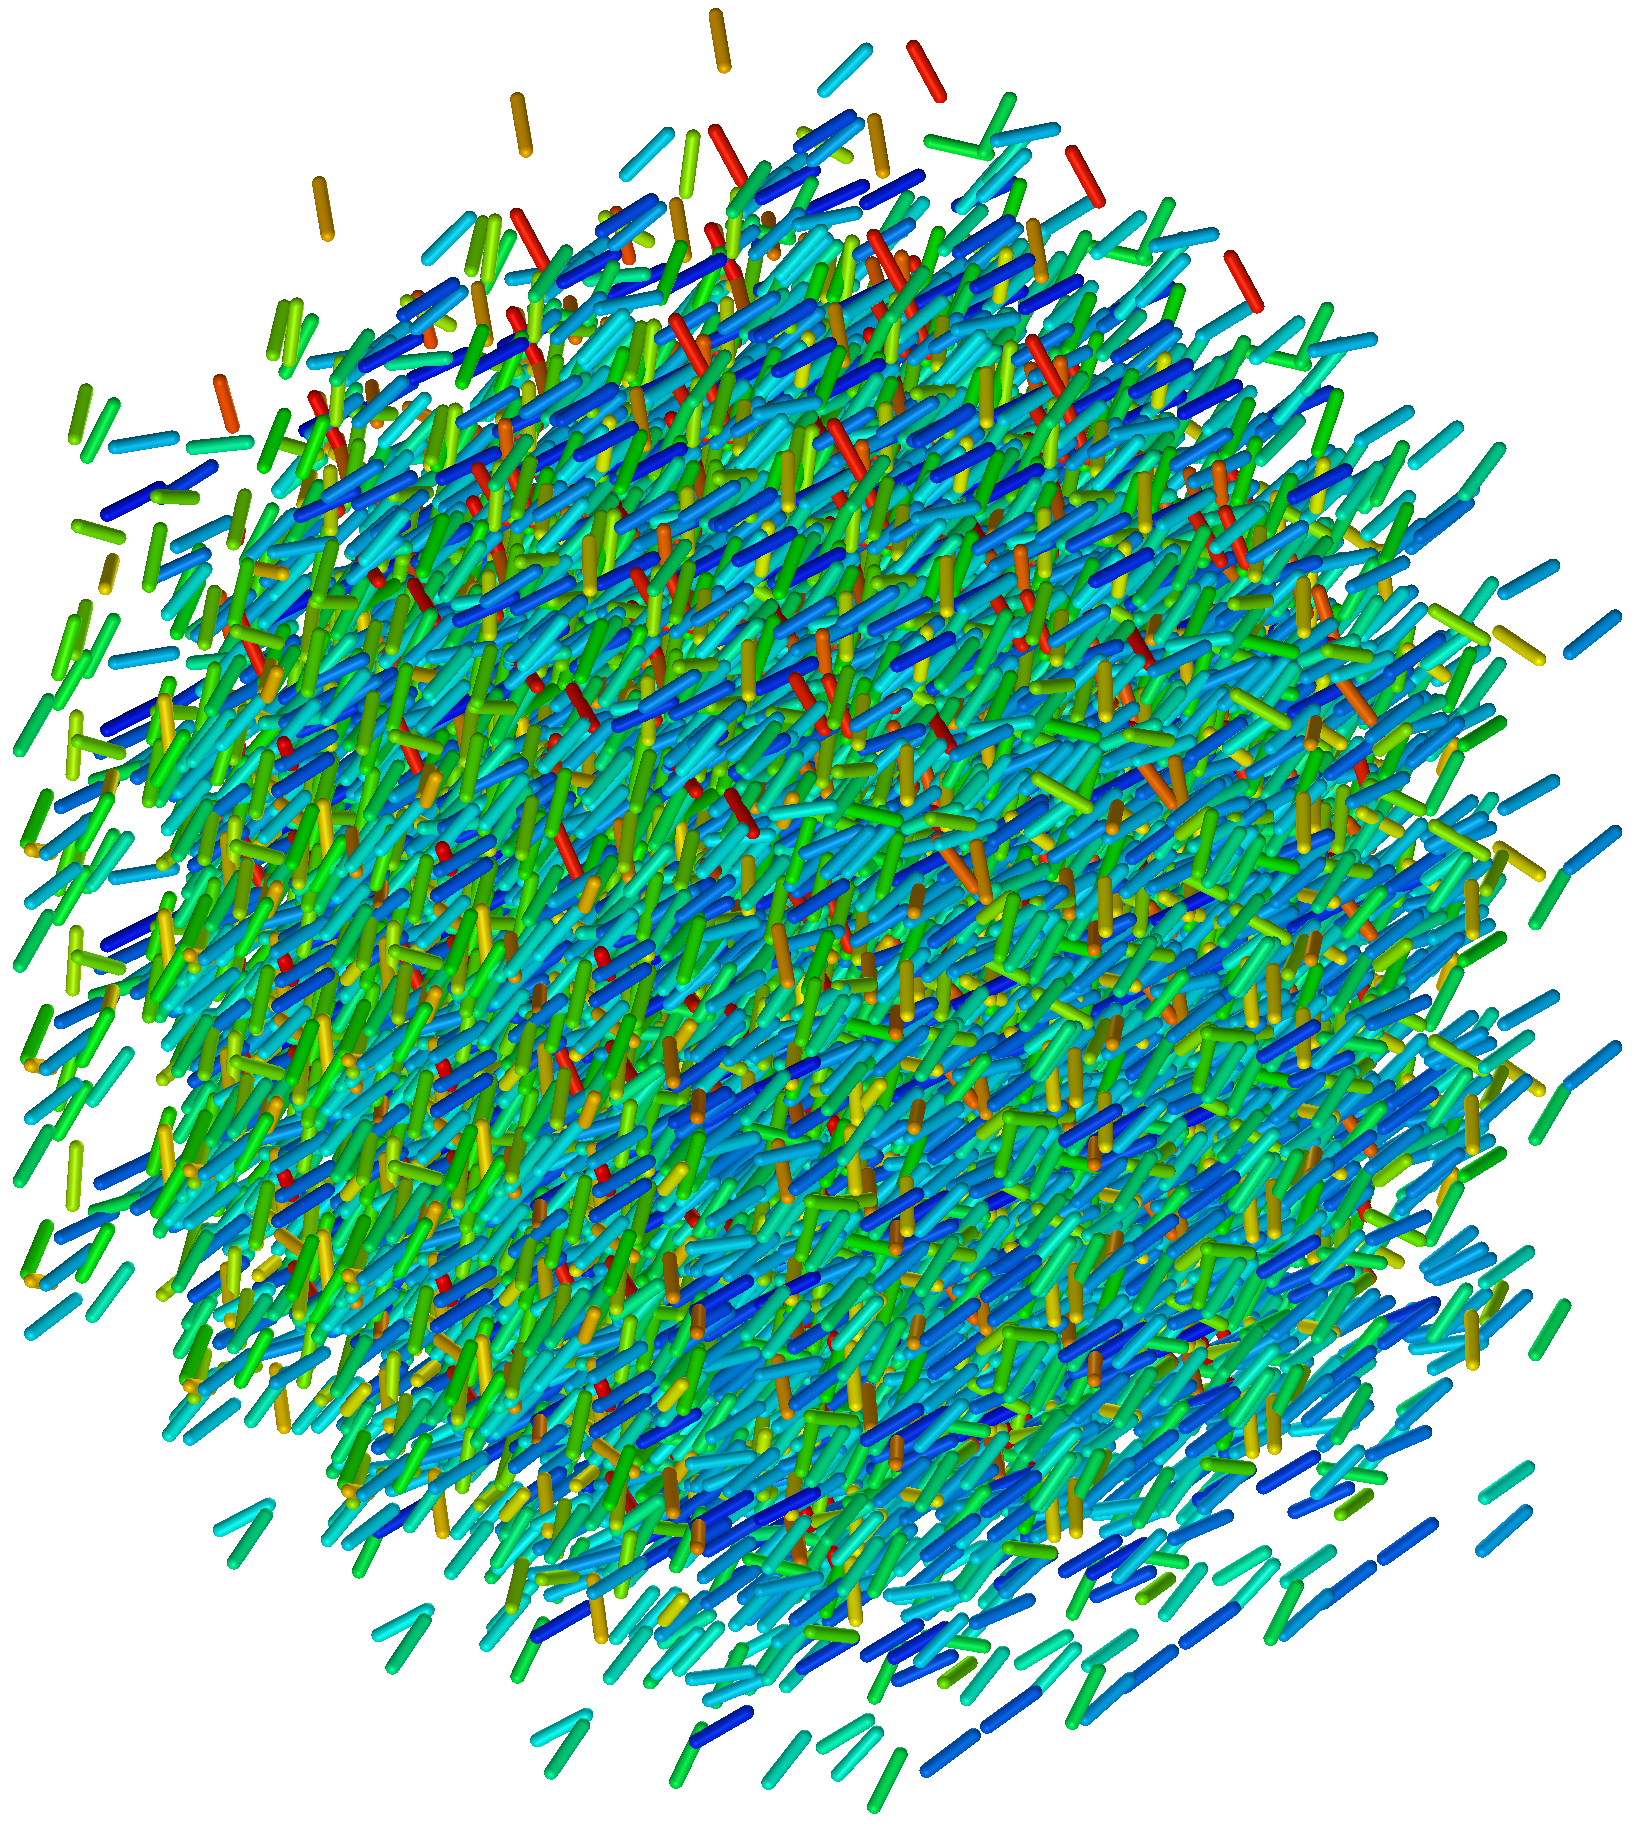
\includegraphics[width=\textwidth]{assets/images/periodic/3}
      \caption{$(1,1,1)$}
      \label{fig:periodic_3}
    \end{subfigure}
  \end{center}
  \caption{Demonstration of periodic repetition of a configuration, labelled with repetition parameter of format $(x, y, z)$.}
  \label{fig:periodic}
\end{figure}

To enable the user to change repetitions, a `Repeats' heading was added to the `Reference' sub menu with X, Y and Z values set to 0 by default. The user can enter any integer value and the configuration updates as need.

\subsection{WebMGA 3.0 Bugs}
TODO
